\chapter{Introdução} % ## 1. Introdução

% <!-- Fazer algumas sutis alterações no português --> 
% <!-- Fazer referência ao TCC do Ricardo falando sobre "Já existem no mercado algumas ferramentas que prometem a geração automatizada de grades de horários" -->
% <!-- Adicionar o que Sanya, Ricardo e Vieira 2011 falam em relação às ferramentas, buscando também um novo autor mais recente que diga o mesmo -->


% <!--    Coisas a dizer
% - A realidade do ensino superior brasileiro
%   - Muitas reprovações
%   - Grade horária confusa
%   - Professores limitados
%   - Preferências diversas     X
%     - Professores             X
%       - Horários              X
%     - Alunos
%       - Estágio               X
%       - Trabalho
%       - Formar rápido
%   - Demanda variada
%   - Caso específico da UENF   X
% -->

No ensino superior brasileiro, cada curso de uma instituição de ensino tem em seu projeto pedagógico, ou seja, no documento que rege quais as atribuições e justificativas de existência do curso, uma listagem de disciplinas a serem ministradas em cada semestre ao longo de sua duração esperada. Disciplinas estas que para serem cursadas os discentes precisam cumprir determinados requisitos. Por exemplo, é esperado que o discente apenas curse a disciplina Cálculo 2 após haver obtido a aprovação prévia na disciplina Cálculo 1.

% <!-- Perguntas
% - Pesquisar quais são as regras que todos os cursos superiores devem seguir para serem reconhecidos pelo MEC
% - Qual a definição de projeto pedagógico?
% - Todos os PPCs dos cursos apresentam a listagem das disciplinas?
% -->

Embora haja este planejamento de duração do curso, diversos fatores podem influenciar esta previsão, dentre eles podemos citar eventos como:

\begin{itemize}
    \item Quebra de pré-requisitos: onde o discente solicita permissão para inscrição em uma disciplina cujos pré-requisitos não são completamente cumpridos por si;
    \item Trancamento de matrícula: onde o discente suspende temporariamente seus estudos na instituição;
    \item Transferência interna: onde o discente migra entre cursos dentro da mesma instituição;
    \item Transferência externa: onde o discente migra entre cursos entre diferentes instituições;
    \item Reprovações: onde o discente não cumpre com o mínimo desempenho esperado na disciplina, geralmente está associado a ausência nas aulas e/ou desempenho inferior ao mínimo esperado nas avaliações;
    \item Disponibilidade de professores: onde os docentes não são suficientes para ministrar todas as disciplinas demandadas pelos discentes em um mesmo semestre.
\end{itemize}

% - Quebra de pré-requisitos: onde o discente solicita permissão para inscrição em uma disciplina cujos pré-requisitos não são completamente cumpridos por si;
% - Trancamento de matrícula: onde o discente suspende temporariamente seus estudos na instituição;
% - Transferência interna: onde o discente migra entre cursos dentro da mesma instituição;
% - Transferência externa: onde o discente migra entre cursos entre diferentes instituições;
% - Reprovações: onde o discente não cumpre com o mínimo desempenho esperado na disciplina, geralmente está associado a ausência nas aulas e/ou desempenho inferior ao mínimo esperado nas avaliações;
% - Disponibilidade de professores: onde os docentes não são suficientes para ministrar todas as disciplinas demandadas pelos discentes em um mesmo semestre.

Estes eventos tendem a, no geral, aumentar o tempo médio para conclusão do curso. Situação em sua maioria indesejada tanto pelos alunos, que mesmo durante seu estudo já visam o mercado de trabalho, quanto pelos professores e a instituição, visto que a evasão do ensino superior brasileiro é um problema existente e estudado a fim de ser minimizado.

% <!--
% - Pesquisar sobre motivos de evasão do ensino superior
% - Adicionar citação
% -->

Com isso, é esperado que a instituição busque alternativas para tornar mais dinâmica e atrativa a experiência dos discentes durante sua jornada. Uma dessas formas é tentando minimizar o impacto que as reprovações nas disciplinas causam nos semestres consecutivos. Para isso sendo então necessária uma análise das disciplinas que devem ser ministradas no próximo semestre, sendo então necessário definir **quais**, **quando**, **onde**, **por quem** e **para quem** serão ministradas. Esta tarefa, entretanto, não é trivial.

\section{Problemáticas} % ### 1.1. Problemáticas

    Embora seja um problema atualmente, isso não significa que seja recente. Desde 1978 \cite{barham_simple_1978} o termo \textit{timetabling} encontra-se no meio acadêmico como o termo referente ao tabelamento de grade horária, sendo assim, é este o termo que será principalmente utilizado neste trabalho. Neste artigo de 1978 já se propunha uma forma para que se obtivesse um tabelamento otimizado, e demonstrava que o método utilizado gerava bons resultados.

    Outra característica é informada por Joshua \cite{thomas_visualization_2009} que fala sobre a multidimensional do problema de timetabling. Por causa dessa questão há uma complexidade elevada para conseguir conceber visual e mentalmente de que forma os dados relacionados ao problema se estruturam, assim dificultando a elaboração de sistemas computacionais que auxiliem nessa tarefa.

    Dada a grande quantidade de variáveis interconectadas e as características específicas de cada instituição \cite{miranda_udpskeduler_2012}, a organização destas informações buscando a melhor solução possível apresenta-se como um desafio. Principalmente se considerarmos que esta solução é, muitas vezes, buscada manualmente, estando também passível de erros humanos como ilustram as Figuras \ref{Academico} e \ref{CCT}.

    % ![Disciplina atribuída no sistema acadêmico à determinada hora e local](img/Falha_de_alocacao/Metodologia-Quinta.png)

    % ![Disciplina não atribuída à determinada hora e local na grade de horários do CCT](img/Falha_de_alocacao/Aulas-CCT-105-2023_1.png)

    \begin{figure}[htbp]\centering
        \caption{\label{Academico}Disciplina atribuída no sistema acadêmico à determinada hora e local}
        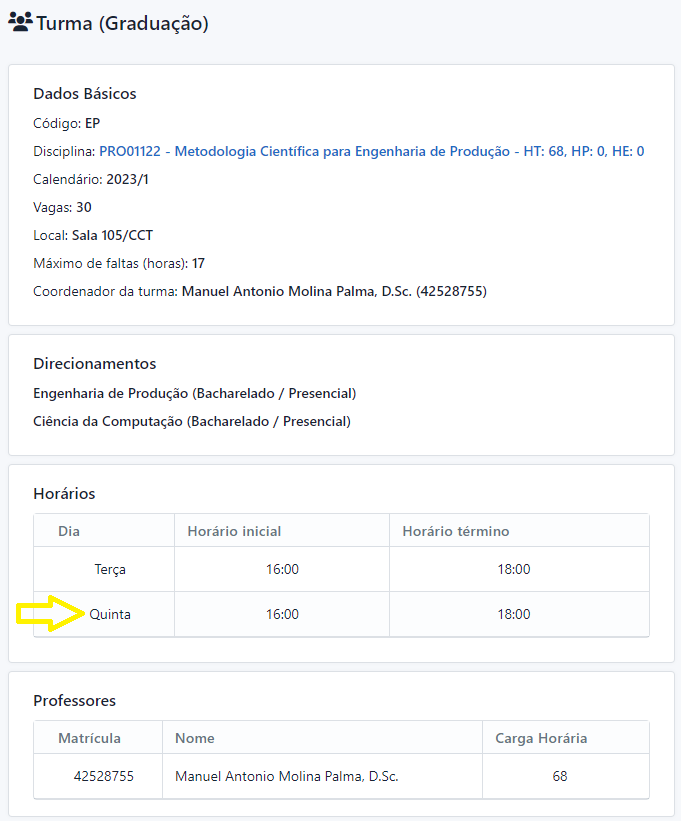
\includegraphics[angle=0,scale=0.8]{files/img/Falha_de_alocacao/Metodologia-Quinta.png}
        \legend{Fonte: o autor}
    \end{figure}    % Imagem acadêmico

    \begin{figure}[htbp]\centering
        \caption{\label{CCT}Disciplina não atribuída à determinada hora e local na grade de horários do CCT}
        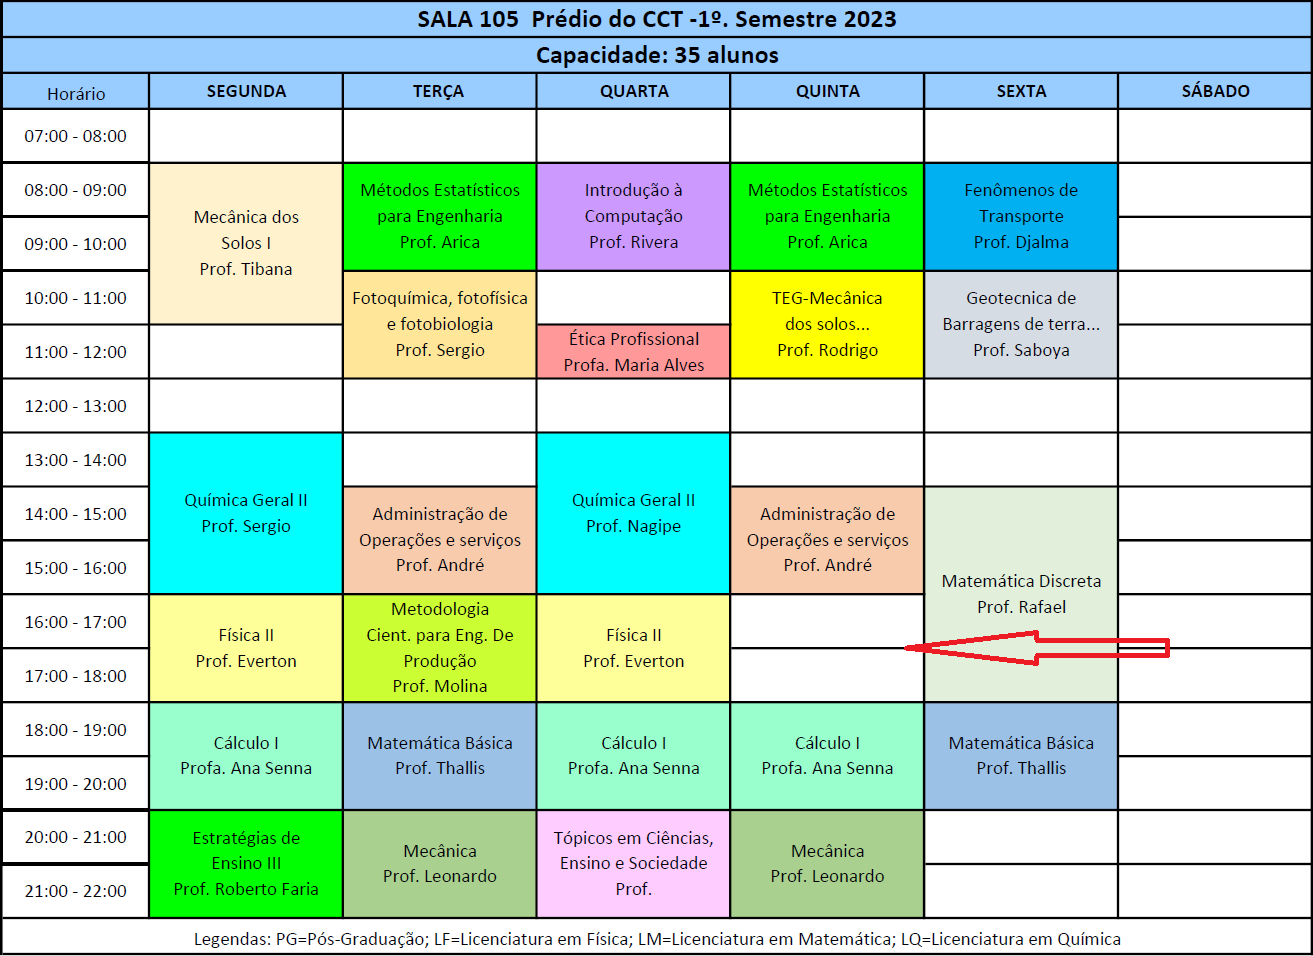
\includegraphics[angle=0,scale=0.5]{files/img/Falha_de_alocacao/Aulas-CCT-105-2023_1.png}
        \legend{Fonte: o autor}
    \end{figure}    % Imagem representando o erro humano na alocação de salas

    Nestas imagens, fica exemplificado um dos possíveis problemas que podem ocorrer durante a criação de grades horárias, que é, mesmo quando uma seção da universidade (o Sistema Acadêmico, ilustrado pela Figura \ref{Academico}) aloca uma turma a uma determinada sala, outra seção da mesma instituição (o Centro de Ciência e Tecnologia, ilustrado pela Figura \ref{CCT}) pode não estar ciente do mesmo, ou mesmo estando ciente pode acabar não delimitando aquela lacuna de tempo como ocupada, assim estando passível de uma segunda alocação naquele período de tempo naquela sala, assim gerando problemas.

    Também segundo J. Miranda, embora o problema de atribuição de salas não seja novo e tenha extensa literatura a seu respeito, são poucos os que de fato implementaram um sistema para suporte de decisões. Isso se dá por diversos fatores, também listado pelo autor fazendo referência a trabalhos anteriores, sendo alguns deles a resistência organizacional a mudanças e adoção de novas tecnologias, nível de dificuldade do problema, dentre outros.

    % <!--  Pegar a referência original? -->

    Algumas outras características que se apresentam como problemas são a falta de otimalidade das grades horárias desenvolvidas em boa parte das instituições de ensino superior e a quantidade de tempo necessária para a criação dessas grades não-ótimas.

    Considerando que situações como a descrita acima são passíveis de ocorrer, e que a tarefa de criação de grades horárias é recorrente, um sistema de suporte à decisão que supra às necessidades dos seus usuários se faz necessário.

\section{Hipótese} % ### 1.2. Hipótese

    Dada as características intrínsecas ao problema de agendamento de grade horária, é esperado que os softwares atualmente existentes que lidam com este problema não apresentem completas capacidades de se moldar ao caso de uma instituição específica.

    E, caso a primeira hipótese se apresente correta, o software a ser desenvolvido, assim como seus similares, se apresentará como uma solução plausível para a resolução do problema proposto embora ainda apresente melhorias possíveis a serem implementadas. O software se apresentará de tal forma que os \textit{stakeholders} que, esperadamente, decidirem não o utilizar não causarão a impossibilidade do uso do sistema.

    % <!--
    %- Os softwares existentes não são adequados para o caso específico
    %- Embora seja possível implementar
    %  - Será trabalhoso
    %  - Precisará atender muitos requisitos
    %  - Nem todos stakeholders aceitarão facilmente a mudança
    %  - O sistema não será tão intuitivo quanto poderia ser
    %  - Muitos não veem essa questão como um problema
    %  - Alguns não acham necessário haver mudança no método de elaboração das grades
    % -->

\section{Objetivos} % ### 1.3. Objetivos

    Os objetivos deste documento podem ser divididos entre gerais e específicos, não havendo relação de superioridade de um em relação ao outro, visto que ambos igualmente nortearão o desenvolvimento da pesquisa.

    \subsection{Gerais} % #### 1.3.1. Gerais

        % <!--
        %- Sistema de suporte à decisão
        %  - Eficiente
        %  - Eficaz
        %  - Efetivo
        %- Criar grades horárias melhores, preferencialmente ótimas
        %- Reduzir tempo necessário para criação das tabelas
        %- Reduzir conflitos
        %- Aumentar satisfação geral com as disciplinas e horários ofertados
        % -->

        Como objetivos gerais, espera-se conseguir desenvolver um sistema de suporte à decisão tal que aumente a eficiência, eficácia e efetividade do processo de criação de grades horárias que semestralmente demandam extensa quantidade de tempo dos coordenadores de curso na UENF e não alcançam a otimalidade. Nesse processo, também é esperado que as grades horárias finais tragam benefícios aos alunos como forma de mais disciplinas à sua disposição. Visto que estes muitas vezes lidam com grades horárias que não contemplam suas reais demandas. Dessa forma aumentando a satisfação de todos os participantes do processo, desde os coordenadores de curso até os alunos.

    \subsection{Específicos} % #### 1.3.2. Específicos

        Como objetivos mais específicos, podemos listar os seguintes:

        \begin{itemize}
            \item Entender de que forma os setores administrativos da UENF atualmente lidam com a questão do \textit{timetabling};
            \item Obter as demandas de aprimoramentos desejadas pelos diferentes centros e laboratórios;
            \item Modelar o sistema de resolução de \textit{timetabling} de acordo com os requisitos demandados;
            \item Encontrar o que é necessário para a adoção da aplicação de tabelamento de horário;
            \item Incentivar o uso de uma ferramenta centralizada para a otimização do \textit{Timetabling Problem}.
        \end{itemize}

        % - Entender de que forma os setores administrativos da UENF atualmente lidam com a questão do \textit{timetabling};
        % - Obter as demandas de aprimoramentos desejadas pelos diferentes centros e laboratórios;
        % - Modelar o sistema de resolução de \textit{timetabling} de acordo com os requisitos demandados;
        % - Encontrar o que é necessário para a adoção da aplicação de tabelamento de horário;
        % - Incentivar o uso de uma ferramenta centralizada para a otimização do \textit{Timetabling Problem}.

\section{Justificativas} % ### 1.4. Justificativas

    Levando em conta a problemática evidenciada e os sucessos prévios dos artigos anteriores, vê-se grande potencial de auxílio e aumento na satisfação de todos os que utilizarem os métodos propostos. Não havendo um sistema geral que solucione todos os casos como evidenciado pelos pesquisadores da área, resta aos interessados rumarem em busca de uma solução entalhada nos moldes de sua instituição específica. Considerando que é um problema existente atualmente e que uma solução está disponível, o que se torna necessário é realizar o esforço inicial suficiente para que ocorra a quebra da inércia em que se encontram os processos ineficientes usuais para assim alcançar um melhor. Sendo assim, faz-se válida a pesquisa e desenvolvimento de um software que vise este propósito.

    % <!--
    % - Levando em conta a problemática e o os sucessos prévios de artigos anteriores
    % - As instituições públicas idealmente deveriam ter um sistema próprio para a resolução de seus próprios conflitos
    % - Não havendo o interesse ou conhecimento geral para este fim, resta aos alunos e pesquisadores interessados buscarem uma solução entalhada nos moldes de sua instituição
    % - Considerando que é um problema existente na instituição e que é resolvível, sendo necessário o esforço inicial de quebrar a inércia dos processos usuais para se alcançar um melhor, faz-se válida a pesquisa e desenvolvimento de um software que vise este propósito.
    % -->

\section{Metodologia } % ### 1.5. Metodologia 

    % <!-- Alterar a parte final da metodologia -->

    % <!--
    % - Entrevistas qualitativas com stakeholders     x
    %   - Adicionar perguntas aqui                    .
    % - Formulário quantitativo com alunos            x
    %   - Adicionar perguntas aqui                    .
    % - Elicitação de requisitos                      x
    %   - Falar sobre o SWEBOK                        x
    % - Desenvolvimento do software                   .
    %   - CI/CD                                       .
    %     - Testes                                    .
    %     - GitHub                                    .
    %   - Programação modular                         SWEBOK
    %   - Obtenção de demanda                         .
    %     - Extratos                                  .
    %       - Processamento e limpeza                 .
    %       - Estruturando dados                      .
    %     - Acadêmico                                 .
    %     - Formulário                                .
    %   - Criando solução inicial                     .
    %   - Otimizando                                  .
    %     - Algoritmos                                .
    %     - Interatividade                            .
    %       - Visualização                            .
    % -->

    Considerando as dificuldades encontradas em trabalhos anteriores, entende-se que o maior desafio será superar as especificidades que serão encontradas durante a modelagem da universidade em questão. Para isso, será inicialmente necessária uma pesquisa bibliográfica com foco no estudo das abordagens qualitativas realizadas anteriormente que obtiveram sucesso em elicitar os requisitos adequados para as instituições de ensino.

    % <!--
    % Adicionar referência sobre pesquisa qualitativa?
    % -->

    Com este conhecimento, um material inicial para a pesquisa exploratória e qualitativa deve ser desenvolvido levando em conta as questões próprias da universidade em questão, visando também coletar dados relevantes para uma futura pesquisa com maior enfoque em características emergentes que a pesquisa anterior pode levantar, similar a como foi proposto e realizado por \cite{andre_interaction_2018}.

    Nesta pesquisa exploratória em formato de entrevista, algumas informações esperadas revolvem em torno das percepções dos \textit{stakeholders} do sistema proposto, sendo esses principalmente os professores, coordenadores de cursos, chefes de laboratório e diretores de centro. Estas percepções incluem o entendimento deles quanto ao método atual e às alternativas existentes, nível de insatisfação com o método atual, nível de desejo quanto à um novo método. Além disso, espera-se aproveitar o ensejo para elicitar as características e funcionalidades que gostariam de ter em um sistema de suporte à decisão, solicitando também que deem informações adicionais que gostariam de acrescentar.

    Essas informações serão relevantes para se atingir a satisfação e uso futuro do sistema proposto. Pois, como é informado no \cite{bourque_swebok_2014}, uma das fontes de requisitos é o ambiente organizacional e como o software muitas vezes visa auxiliar em algum processo da instituição, processo este já condicionado à sua estrutura, cultura e políticas externas, o engenheiro de software precisa estar atento a elas, visto que o novo software não deve forçar mudanças não planejadas em processos de negócios.

    Questionamentos similares também serão realizados com alunos, porém em formato de formulário online para facilitar o processamento dos dados coletados.

    % <!--
    \def\LinkParadigm{https://www.visual-paradigm.com/}
    \def\LinkDrawio{https://www.drawio.com/}
    \def\LinkMermaid{https://mermaid.js.org/}
    % -->

    % [LinkDrawio]: https://www.drawio.com/
    % [LinkMermaid]: https://mermaid.js.org/
    % [LinkVisualParadigm]: https://www.visual-paradigm.com/

    Tendo obtido as informações dos \textit{stakeholders} primários, será então necessário modelar quais são as regras que ditam a estrutura organizacional em foco. Para este fim, serão utilizados diagramas conceituais utilizando softwares de suporte como o [Visual Paradigm][LinkVisualParadigm], [draw.io][LinkDrawio] e a [ferramenta Mermaid][LinkMermaid].

    % <!--
    % Essa parte de baixo está muito estranha. Revisar depois
    % -->

    Esta etapa será de grande importância pois guiará a pesquisa para quais serão os detalhes dos módulos existentes durante o desenvolvimento do projeto, bem como esclarecerá visualmente quais são as informações sobre os recursos que são necessárias para se calcular a grade ótima. Como por exemplo:

    % <!--

    \begin{enumerate}
        \item Salas
        \begin{enumerate}
            \item Quais são as salas disponíveis?
            \item Quais as capacidades de cada um?
            \item Em quais horários estão disponíveis?
            \item Quais são suas peculiaridades?
            \begin{enumerate}
                \item Têm computadores?
                \item Têm quadro?
                \item Têm televisão?
                \item Têm projetor?
            \end{enumerate}
        \end{enumerate}
        \item Alunos
        \begin{enumerate}
            \item Quantos são?
            \item Quais matérias demandam?
        \end{enumerate}
        \item Professores
        \begin{enumerate}
            \item Quais disciplinas ministram?
            \item Quantas disciplinas podem ministrar?
            \item Quais seus horários de preferência?
        \end{enumerate}
    \end{enumerate}
    % -->

    % - Salas
    %   - Quais são as salas disponíveis?
    %   - Quais as capacidades de cada um?
    %   - Em quais horários estão disponíveis?
    %   - Quais são suas peculiaridades?
        % - Têm computadores?
        % - Têm quadro?
        % - Têm televisão?
        % - Têm projetor?
    % - Alunos
    %   - Quantos são?
    %   - Quais matérias demandam?
    % - Professores
    %   - Quais disciplinas ministram?
    %   - Quantas disciplinas podem ministrar?
    %   - Quais seus horários de preferência?


    % <!-- Realmente vou testar? -->

    Com as regras organizacionais e variáveis bem definidas, serão testados alguns softwares que visam a criação de grades horárias para confirmar se há a real necessidade de se desenvolver um software específico para a instituição. Após realizados os testes, caso os softwares existentes supram as necessidades, este será utilizado nos passos seguintes. De outro modo, haverá a necessidade de desenvolvimento de um sistema de suporte à decisão como ferramenta centralizada para este fim.

    Independente de qual dos softwares será testada a aplicabilidade do mesmo no contexto universitário e será mensurada a satisfação dos \textit{stakeholders} durante o seu uso, assim buscando assegurar o seu uso na criação de grades horárias ótimas futuras.

\section{Estrutura/Organização} % ### 1.6. Estrutura/Organização

    Este trabalho abordará capítulos que de forma resumida lidam com os seguintes tópicos:

    \begin{itemize}
        \item O capítulo 1 de introdução traça informações gerais sobre o assunto do trabalho, elaborando mais detalhadamente quanto à sua problemática, hipótese, objetivos, justificativas, a metodologia escolhida e a organização de suas informações;
        \item O capítulo 2 de revisão literária informa mais detalhadamente sobre os problemas de agendamento, suas categorias, soluções, desafios e definições de termos;
        \item O capítulo 3 de desenvolvimento apresenta as informações coletadas durante as entrevistas. Apresenta também a estrutura geral dos códigos feitos, principalmente ilustrando quais os comportamentos esperados em cada um dos módulos, bem como quais foram as ferramentas utilizadas e as práticas seguidas;
        \item O Capítulo 4 de resultados e discussões demonstra o software final utilizado, apresenta comparações das qualidades entre grades horárias geradas pelo software e as que foram utilizadas nos últimos semestres. Apresenta também a pesquisa de satisfação realizada com os \textit{stakeholders} entrevistados no início do desenvolvimento;
        \item O Capítulo 5 da conclusão e trabalhos futuros finaliza o presente trabalho com os pensamentos gerais sobre a pesquisa e desenvolvimento, apresentando as características não abordadas e indicando caminhos a serem seguidos por pesquisadores posteriormente.
    \end{itemize}

    % - O capítulo 1 de introdução traça informações gerais sobre o assunto do trabalho, elaborando mais detalhadamente quanto à sua problemática, hipótese, objetivos, justificativas, a metodologia escolhida e a organização de suas informações;
    % - O capítulo 2 de revisão literária informa mais detalhadamente sobre os problemas de agendamento, suas categorias, soluções, desafios e definições de termos;
    % - O capítulo 3 de desenvolvimento apresenta as informações coletadas durante as entrevistas. Apresenta também a estrutura geral dos códigos feitos, principalmente ilustrando quais os comportamentos esperados em cada um dos módulos, bem como quais foram as ferramentas utilizadas e as práticas seguidas;
    % - O Capítulo 4 de resultados e discussões demonstra o software final utilizado, apresenta comparações das qualidades entre grades horárias geradas pelo software e as que foram utilizadas nos últimos semestres. Apresenta também a pesquisa de satisfação realizada com os \textit{stakeholders} entrevistados no início do desenvolvimento;
    % - O Capítulo 5 da conclusão e trabalhos futuros finaliza o presente trabalho com os pensamentos gerais sobre a pesquisa e desenvolvimento, apresentando as características não abordadas e indicando caminhos a serem seguidos por pesquisadores posteriormente.
